\documentclass{article}

% if you need to pass options to natbib, use, e.g.:
% \PassOptionsToPackage{numbers, compress}{natbib}
% before loading nips_2018

% ready for submission
\usepackage[final]{nips_2018}

% to compile a preprint version, e.g., for submission to arXiv, add
% add the [preprint] option:
% \usepackage[preprint]{nips_2018}

% to compile a camera-ready version, add the [final] option, e.g.:
% \usepackage[final]{nips_2018}

% to avoid loading the natbib package, add option nonatbib:
% \usepackage[nonatbib]{nips_2018}

\usepackage[utf8]{inputenc} % allow utf-8 input
\usepackage[T1]{fontenc}    % use 8-bit T1 fonts
\usepackage{hyperref}       % hyperlinks
\usepackage{url}            % simple URL typesetting
\usepackage{booktabs}       % professional-quality tables
\usepackage{amsfonts}       % blackboard math symbols
\usepackage{nicefrac}       % compact symbols for 1/2, etc.
\usepackage{microtype}      % microtypography
\usepackage[vlined,ruled,commentsnumbered,linesnumbered]{algorithm2e}
\usepackage[fleqn]{amsmath}
\usepackage{listings}
\usepackage{graphicx}
\usepackage{subfigure}
\usepackage{color,xcolor}
% \usepackage{fontspec}
% \setmainfont{Times New Roman}

\title{CS420 Project Report}

% The \author macro works with any number of authors. There are two
% commands used to separate the names and addresses of multiple
% authors: \And and \AND.
%
% Using \And between authors leaves it to LaTeX to determine where to
% break the lines. Using \AND forces a line break at that point. So,
% if LaTeX puts 3 of 4 authors names on the first line, and the last
% on the second line, try using \AND instead of \And before the third
% author name.

\author{
  Ruiheng Chang \\
  515021910459\\
  Department of Computer Science\\
  Shanghai Jiao Tong University\\
  \texttt{crh19970307@sjtu.edu.cn}
  \And
  Weichao Mao \\
  515021910559\\
  Department of Computer Science\\
  Shanghai Jiao Tong University\\
  \texttt{maoweichao@sjtu.edu.cn}
  %% \AND
  %% Coauthor \\
  %% Affiliation \\
  %% Address \\
  %% \texttt{email} \\
  %% \And
  %% Coauthor \\
  %% Affiliation \\
  %% Address \\
  %% \texttt{email} \\
  %% \And
  %% Coauthor \\
  %% Affiliation \\
  %% Address \\
  %% \texttt{email} \\
}

\begin{document}
% \nipsfinalcopy is no longer used

\maketitle

\section{Traditional Models}
In this section, we first preprocess the images on the pixel level to remove the disturbances. We then perform traditional classification models, such as KNN and SVM, on the processed images. We further compare the performance of the traditional models with and without the preprocessing procedure. Finally, we employ ensemble methods and try to obtain better predictive performance.

\subsection{Pixel-Level Image Preprocessing}
We can easily see the data set given to us is generated by adding some minor disturbances to the standard MNIST data set. These disturbances include shifting of the main digit, and small random pepper noise which presents itself as sparsely occurring white pixels. 

Before applying traditional machine learning algorithms on the disturbed MNIST data set, we first perform pixel-level preprocessing on the images, aiming to reverse the disturbances and reconstruct the original images. In the following, we will demonstrate our preprocessing procedure step by step.

\subsubsection{Timeline Overview}
The preprocessing steps are summarized in Figure~\ref{fig:preoverview}. Figure\ref{subfig:original} shows one original image from the given data set. As we can see, there is a patch of white noise on the right side, and the digit is located in the lower half of the image. Our first step in the preprocessing removes the white noise on the right, and the denoised result is shown in Figure\ref{subfig:denoised}. In the second step, we crop out the minimum rectangle that covers the digit pixels, and Figure~\ref{subfig:cropped} shows the cropped digit. Finally, Figure~\ref{subfig:centered} shows the centered image after we add equal padding to the digit. 

\begin{figure}[!htb]
	\centering
	\subfigure[Original]{
	\label{subfig:original}
	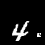
\includegraphics[width=.2\textwidth]{fig//3_original.png}
}
	\subfigure[Denoised]{
	\label{subfig:denoised}
	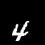
\includegraphics[width=.2\textwidth]{fig//3_denoised.png}	
}
\subfigure[Cropped]{
	\label{subfig:cropped}
	
\includegraphics[width=.18\textwidth]{fig//3_cropped.png}	
}
\subfigure[Centered]{
\label{subfig:centered}

\includegraphics[width=.2\textwidth]{fig//3_centered.png}	
}
\caption{Preprocessing timeline overview.}
\label{fig:preoverview}
\end{figure}

\subsubsection{Step 1: Denoising}
The first step concerns searching and removing the white pepper noise in the image. In this step, we regard any white pixel block with no more than 20 pixels as the noise area. The intuition is, the pixels of digits 0 to 9 are all connected blocks, and since the digit is the main part in the image, it must contain a large area of pixels (more than 20 pixels). 

We utilize the simple Depth First Search (DFS) algorithm to search for the connected blocks. We enumerate each of the pixels in the image from the upper-left corner. If the current pixel is a white pixel, we will further check its 8 neighboring pixels and if there exist white pixels among its neighbors, we connect them into a single block. Figure\ref{fig:DFS} demonstrates the detailed process of this step. Suppose the original binary image is shown in Figure\ref{subfig:binary}. For a white pixel we are visiting (colored in blue in Figure\ref{subfig:neighbors}), we need to further check its 8 neighbors. Since we find two more white pixels among its neighbors (colored in yellow in Figure\ref{subfig:neighbors}), we connect the three pixels into a single block, and repeat the same procedure on the two neighboring white pixels. Finally, we will find the whole white connected block. 

\begin{figure}[!htb]
	\centering
	\subfigure[Original image]{
		\label{subfig:binary}
		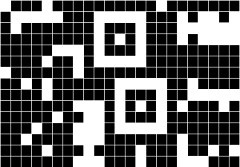
\includegraphics[width=.45\textwidth]{fig//DFS1}
	}
	\hspace{.2in}
	\subfigure[Neighbors]{
		\label{subfig:neighbors}
		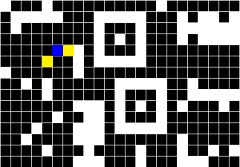
\includegraphics[width=.45\textwidth]{fig//DFS2}	
	}
	\caption{White block searching.}
	\label{fig:DFS}
\end{figure}

Once we have found the noise area (i.e., the white connected blocks with area no more than 20 pixels), the denoising process is easy to implement. We only need to employ the Flood Fill algorithm on the noise areas, and color the white pixels into black. A different statement of the same process is to perform a second DFS on the noise pixels, and color every white pixel we visit into black. 

\subsubsection{Step 2: Cropping}

So far, we have safely removed the white pepper noises from the images, but we still cannot feed the current digit into the traditional models directly. The problem is, the digits are not centered in the image, and although some models like convolutional neural networks are not sensitive to shifting, these misaligned digits can rule out many traditional models like KNN. To guarantee a reasonable performance of the traditional models, we further need to center the digital pixels right in the middle of the image.

This second step is relatively easy. We only need to find the boundaries of the digit and crop it out. As illustrated in Figure\ref{fig:crop}, we can enumerate to find the upper-most, left-most, right-most and lower-most pixels in the denoised image, and use these pixels as boundaries (denoted by yellow lines in Figure\ref{subfig:bar}) to crop out the digital area.

\begin{figure}[!htb]
	\centering
	\subfigure[Boundaries]{
		\label{subfig:bar}
		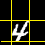
\includegraphics[width=.2\textwidth]{fig//3_denoised_bar}	
	}
\hspace{.2in}
\subfigure[Cropped digit]{
	\label{subfig:cropped2}
	
\includegraphics[width=.18\textwidth]{fig//3_cropped.png}	
}
	\caption{Cropping out the digit.}
	\label{fig:crop}
\end{figure}

\subsubsection{Step 3: Centering}
Finally, we will center the digital area right in the middle of the image. We want to keep the size of the image ($45\times 45$) unchanged before and after the preprocessing procedure so that we can simply feed the new data set into our previous models. Since the size of the cropped image can be a little smaller than the original image, we add equal padding to the left, right, up and down side of the digit to make its size equal to the original one. The equal padding also guarantees the digit will always be centered in the image, so that the misalignment of digits is not a problem anymore. The OpenCV library provides a function \textit{copyMakeBorder} that implements this operation. Therefore, we only need to calculate the padding length and then safely rely on OpenCV to do the padding job. 

So far, we have finished our preprocessing steps, and the images are ready to be feed into the traditional models. For more detailed explanations of these preprocessing steps, please refer to the comments in our code in file \texttt{preprocessing.py}.

\subsection{K-Nearest Neighbors}





\bibliographystyle{ieee}
\bibliography{egbib}
\end{document}
